\Opensolutionfile{ans}[ans/ans-2H3-TL-1]
\setcounter{chapter}{2}
\chap{PHƯƠNG PHÁP TỌA ĐỘ TRONG KHÔNG GIAN}
\section{HỆ TỌA ĐỘ TRONG KHÔNG GIAN}
\subsection{Tóm tắt lý thuyết}
\begin{tomtat}
	\subsubsection{Hệ trục tọa độ trong không gian}
	Trong không gian, xét ba trục tọa độ $Ox, Oy, Oz$ vuông góc với nhau từng đôi một và chung một điểm gốc $O$. Gọi $\overrightarrow{i}, \overrightarrow{j}, \overrightarrow{k}$ là các vec-tơ đơn vị, tương ứng trên các trục $Ox, Oy, Oz$. Hệ ba trục như vậy gọi là hệ trục tọa độ vuông góc trong không gian.
	\begin{center}
		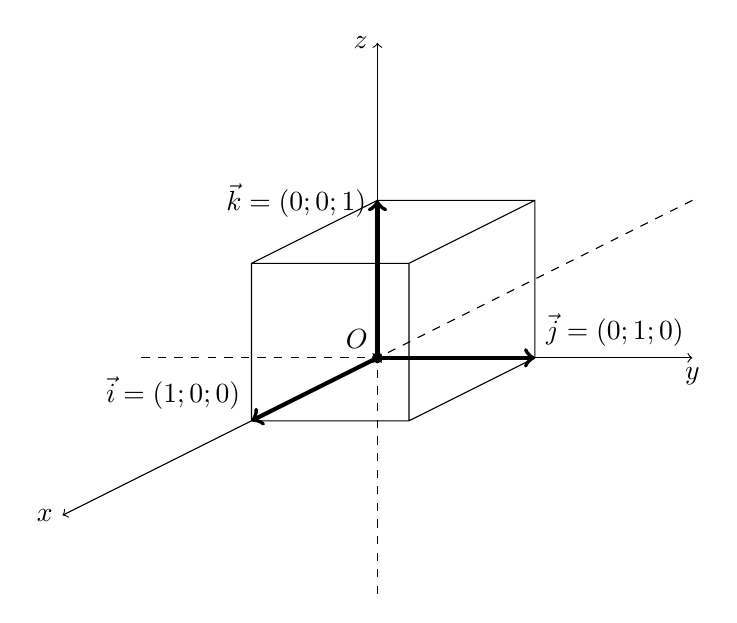
\begin{tikzpicture}
		\draw[->,dashed] (-3,0)--(0,0);
		\draw[->](0,0)--(4,0)node[below]{$y$};
		\draw[->, line width=1.5pt](0,0)--(2,0) node[above right]{$\vec{j}=(0;1;0)$};
		\draw[->,dashed] (0,-3)--(0,0);
		\draw[->](0,0)--(0,4)node[left]{$z$};
		\draw[->, line width=1.5pt](0,0)--(0,2) node[left]{$\vec{k}=(0;0;1)$};
		\draw[->,dashed] (4,2)--(0,0);
		\draw[->](0,0)--(-4,-2)node[left]{$x$};
		\draw[->, line width=1.5pt](0,0)--(-1.6,-.8) node[above left]{$\vec{i}=(1;0;0)$};
		\draw (0,0) node[above left] {$O$} ;
		\fill (0,0) circle (2pt);
		\draw (-1.6,-.8)--(-1.6,1.2)--(0,2)--(2,2)--(2,0)--(0.4,-0.8)--(-1.6,-0.8) (-1.6,1.2)--(0.4,1.2)--(2,2) (0.4,1.2)--(0.4,-0.8);
		\end{tikzpicture}
	\end{center}

\begin{itemize}
\item Điểm $O$ gọi là gốc tọa độ.
\item Trục $Ox$ gọi là trục hoành; Trục $Oy$ gọi là trục tung; Trục $Oz$ gọi là trục cao.
\item Các mặt phẳng chứa hai trục tọa độ gọi là các mặt phẳng tọa độ. Ta kí hiệu chúng lần lượt là $\left(Oxy\right)$, $\left(Oyz\right)$, $\left(Ozx\right)$.
\item Véc-tơ đơn vị của trục $Ox$, $Oy$, $Oz$ lần lượt là: $\vec{i}$, $\vec{j}$, $\vec{k}$.
\item Các véc tơ đơn vị đôi một vuông góc với nhau và có độ dài bằng 1:
${\vec{i}}^2={\vec{j}}^2={\vec{k}}^2=1$  và $\vec{i}.\vec{j}=\vec{j}.\vec{k}=\vec{i}.\vec{k}=0$
\end{itemize}
	\subsubsection{Tọa độ của véc-tơ}
	\begin{dn}
		$\vec{u}=(x;y;z)\Leftrightarrow \vec{u}=x\vec{i}+y\vec{j}+z\vec{k}$ với $\vec{i}$, $\vec{j}$, $\vec{k}$ là các véc-tơ đơn vị, tương ứng trên các trục $Ox$, $Oy$, $Oz$.
		
	\end{dn}
	\begin{tc}
		Cho hai véc-tơ $\vec{a}=(a_1;a_2;a_3 )$, $\vec{b}=(b_1;b_2;b_3)$ và $k$ là số thực tùy ý, ta có
		\begin{enumerate}
			\item $\vec{a}+\vec{b}=(a_1+b_1;a_2+b_2;a_3+b_3 )$.
			\item $\vec{a}-\vec{b}=(a_1-b_1;a_2-b_2;a_3-b_3 )$.
			\item $k\cdot \vec{a}=(ka_1;ka_2;ka_3 )$.
			\item $\vec{a}=\vec{b}\Leftrightarrow \left\{ \begin{matrix}
			a_1=b_1 \\
			a_2=b_2 \\
			a_3=b_3. \\
			\end{matrix} \right.$
			\item $\vec{a}$ cùng phương $\vec{b}$, $(\vec{b}\ne \vec{0} )\Leftrightarrow  \heva{
				& a_1=kb_1 \\
				& a_2=kb_2 \\
				& a_3=kb_3 \\
			}\Leftrightarrow  \dfrac{a_1}{b_1}=\dfrac{a_2}{b_2}=\dfrac{a_3}{b_3}$ với $ b_1$,  $b_2$, $b_3\ne 0$.
			\item $\vec{a}\cdot \vec{b}=a_1\cdot b_1+a_2\cdot b_2+a_3\cdot b_3$.
			\item $\vec{a}\perp \vec{b}\Leftrightarrow \vec{a}\cdot \vec{b}=0\Leftrightarrow a_1\cdot b_1+a_2\cdot b_2+a_3\cdot b_3=0$.
			\item $\vec{a}^2=a_1^2+a_2^2+a_3^2$, suy ra $\left| \vec{a} \right|=\sqrt{\vec{a}^2}=\sqrt{a_1^2+a_2^2+a_3^2}$.
			\item $\cos (\vec{a};\vec{b} )=\dfrac{\vec{a}\cdot \vec{b}}{\left| \vec{a} \right|\cdot \left| \vec{b} \right|}=\dfrac{a_1b_1+a_2b_2+a_3b_3}{\sqrt{a_1^2+a_2^2+a_3^2}\cdot \sqrt{b_1^2+b_2^2+b_3^2}}$ với $\vec{a}\ne \vec{0}$, $\vec{b}\ne \vec{0}$.
			
		\end{enumerate}
	\end{tc}
	\subsubsection{Tọa độ của điểm}
	\begin{dn}
		$M(x; y; z )\Leftrightarrow \vec{OM} = (x; y; z )\Leftrightarrow \vec{OM}= x\vec{i}+y\vec{j}+z\vec{k}$ ($x$: hoành độ, $y$: tung độ, $z$: cao độ).
	\end{dn}
	\textbf{Chú ý:} Trong hệ tọa độ $Oxyz$, cho điểm $M(x;y;z )$ ta có các khẳng định sau:
	\begin{enumerate}
		\item $M\equiv O\Leftrightarrow M(0;0;0 )$.
		\item $M\in (Oxy )\Leftrightarrow z=0$, tức là $M(x;y;0 )$
		\item $M\in (Oyz )\Leftrightarrow x=0$, tức là $M(0;y;z )$
		\item $M\in (Oxz )\Leftrightarrow y=0$, tức là $M(x;0;z )$
		\item $M\in Ox\Leftrightarrow y=z=0$, tức là $M(x;0;0 )$
		\item $M\in Oy\Leftrightarrow x=z=0$, tức là $M(0;y;0 )$
		\item $M\in Oz\Leftrightarrow x=y=0$, tức là $M(0;0;z )$
	\end{enumerate}
	\begin{tc}
		Cho bốn điểm không đồng phẳng
		$A(x_A;y_A;z_A )$, $B(x_B;y_B;z_B )$, $C(x_C;y_C;z_C )$ và $D(x_D;y_D;z_D )$.
		
		\begin{enumerate}
			\item $\vec{AB}=(x_B-x_A;y_B-y_A;z_B-z_A )$.
			\item $AB=\left| \vec{AB} \right|=\sqrt{(x_B-x_A)^2+(y_B-y_A )^2+(z_B-z_A )^2}$.
			\item  Tọa độ trung điểm $I$ của đoạn thẳng $AB$ là
			\begin{center}
				$I\left(\dfrac{x_A+x_B}{2};\dfrac{y_A+y_B}{2};\dfrac{z_A+z_B}{2} \right)$.
			\end{center}
			\item Tọa độ trọng tâm $G$ của tam giác $ABC$ là
			\begin{center}
				$G\left(\dfrac{x_A+x_B+x_C}{3};\dfrac{y_A+y_B+y_C}{3};\dfrac{z_A+z_B+z_C}{3} \right)$.
			\end{center}
			\item Tọa độ trọng tâm $G$ của tứ diện $ABCD$ là
			\begin{center}
				$G\left(\dfrac{x_A+x_B+x_C+x_D}{4};\dfrac{y_A+y_B+y_C+y_D}{4};\dfrac{z_A+z_B+z_C+z_D}{4} \right)$.
			\end{center}
		\end{enumerate}
	\end{tc}
	\subsubsection{Phương trình mặt cầu}
	\begin{enumerate}
		\item Mặt cầu tâm $I(a;b;c )$, bán kính $R$ có phương trình
		$(S )\colon (x-a )^2+(y-b )^2+(z-c )^2=R^2$.
		\item Xét phương trình $x^2+y^2+z^2+2ax+2by+2cz+d=0$. $(* )$
		Ta có \begin{eqnarray*}
			(* )&\Leftrightarrow& (x^2+2ax )+(y^2+2by )+(z^2+2cz )=-d\\
			&\Leftrightarrow& (x+a )^2+(y+b )^2+(z+c )^2=-d+a^2+b^2+c^2.
		\end{eqnarray*}
		Để phương trình $(* )$ là phương trình mặt cầu $\Leftrightarrow a^2+b^2+c^2>d$.\\ Khi đó $(S )$ có
		$\heva{
			& \text{tâm }I(-a;-b;-c ) \\
			& \text{bán kính }R=\sqrt{a^2+b^2+c^2-d}. \\
		}.$
		\item Đặc biệt: $(S )\colon x^2+y^2+z^2=R^2$, suy ra $(S )$ có $\heva{
			& \text{tâm }O(0;0;0 ) \\
			& \text{bán kính }R. \\
		}$
	\end{enumerate}
	\end{tomtat}

\subsection{Các dạng bài tập và phương pháp giải}
\begin{dang}{Tìm tọa độ điểm, véc-tơ liên quan đến hệ trục $Oxyz$}
	\begin{itemize}
		\item Áp dụng các công thức tọa độ vec-tơ.
		\item Áp dụng các công thức tọa độ điểm.
	\end{itemize}
\begin{note}
	\textbf{Chú ý:}   Xét tam giác $ABC$, ta có các điểm đặc biệt sau:
	\begin{itemize}
		\item Tọa độ trọng tâm tam giác $ABC$ là $G\left(\dfrac{x_A + x_B + x_C}{3}; \dfrac{y_A + y_B + y_C}{3}; \dfrac{z_A + z_B + z_C}{3}\right)$.
		\item $A'$ là chân đường cao kẻ từ $A$ của tam giác $ABC$ $\Leftrightarrow \heva{&\overrightarrow{AA'} \perp \overrightarrow{BC} \\&\overrightarrow{BA'} \text{ và } \overrightarrow{BC} \text{ cùng phương.}}$
		\item $H$ là trực tâm tam giác $ABC$ $\Leftrightarrow \heva{&\overrightarrow{AH} \perp \overrightarrow{BC} \\&\overrightarrow{BH} \perp \overrightarrow{AC} \\&\overrightarrow{AH}, \overrightarrow{AB}, \overrightarrow{AC} \text{ đồng phẳng.}}$
		\item $D$ là chân đường phân giác trong của góc $A$ của tam giác $ABC$ $\Leftrightarrow \overrightarrow{DB} = -\dfrac{AB}{AC}\overrightarrow{DC}$.
		\item $E$ là chân đường phân giác ngoài của góc $A$ của tam giác $ABC$ $\Leftrightarrow \overrightarrow{EB} = \dfrac{AB}{AC}\overrightarrow{EC}$.
		\item $I$ là tâm đường tròn ngoại tiếp tam giác $ABC$ $\Leftrightarrow \heva{&IA = IB = IC \\&\overrightarrow{AI}, \overrightarrow{AB}, \overrightarrow{AC} \text{ đồng phẳng.}}$
		\item $J$ là tâm đường tròn nội tiếp tam giác $ABC$ $\Leftrightarrow J$ là chân đường phân giác trong của góc $B$ của tam giác $ABD$, với $D$ là chân đường phân giác trong của góc $A$ của tam giác $ABC$.
	\end{itemize}
\end{note}
\end{dang}
\subsubsection{VÍ DỤ MINH HỌA}
\setcounter{vd}{0}
\begin{vd}%[Đỗ Đường Hiếu]%[2H3B1]
	Trong không gian $Oxyz$, cho các véc-tơ $\overrightarrow{a}=(5;-7;2)$, $\overrightarrow{b}=(0;3;4)$, $\overrightarrow{c}=(-1;2;3)$. Tìm tọa độ các véc-tơ $\overrightarrow{u}=2\overrightarrow{a}-\overrightarrow{b}$, $\overrightarrow{v}=3\overrightarrow{a}+4\overrightarrow{b}+2\overrightarrow{c}$.
	\loigiai{
		\begin{itemize}
			\item Ta có ${ \left\{\begin{aligned}&2\overrightarrow{a}=(10;-14;4)\\&-\overrightarrow{b}=(0;-3;-4)\end{aligned}\right.}\Rightarrow  \overrightarrow{u}=2\overrightarrow{a}-\overrightarrow{b} =(10;-17;0)$. Vậy $\overrightarrow{u}=(10;-17;0)$.
			\item ${ \left\{\begin{aligned}&3\overrightarrow{a}=(15;-21;6)\\&4\overrightarrow{b}=(0;12;16)\\&2\overrightarrow{c}=(-2;4;6)\end{aligned}\right.}\Rightarrow  \overrightarrow{v}=3\overrightarrow{a}+4\overrightarrow{b}+2\overrightarrow{c}=(13;-7;28)$. Vậy $\overrightarrow{v}=(13;-7;28)$.
		\end{itemize}
	}
\end{vd}
\begin{vd}%[Đỗ Đường Hiếu]%[2H3B1]%[2H3K1]
	Trong không gian $Oxyz$, cho các véc-tơ $\overrightarrow{u}=3\overrightarrow{i}-2\overrightarrow{j}+\overrightarrow{k}$, $\overrightarrow{v}=-\dfrac{3}{2}\overrightarrow{i}+\overrightarrow{j}-\dfrac{1}{2}\overrightarrow{k}$, $\overrightarrow{w}=6\overrightarrow{i}+m\overrightarrow{j}-n\overrightarrow{k}$.
	\begin{enumerate}
		\item Chứng minh $\overrightarrow{u}$ và $\overrightarrow{v}$ cùng phương.
		\item Tìm $m$ và $n$ để véc-tơ $\overrightarrow{u}$ và $\overrightarrow{w}$ cùng phương.
	\end{enumerate}
	\loigiai{
		Ta có $\overrightarrow{u}=(3;-2;1)$, $\overrightarrow{v}=\left(-\dfrac{3}{2}; 1; -\dfrac{1}{2}\right)$, $\overrightarrow{w}=\left(6; m; -n\right)$.
		\begin{enumerate}
			\item Hai véc-tơ $\overrightarrow{u}$ và $\overrightarrow{v}$ cùng phương khi và chỉ khi 
			$$\overrightarrow{v}=k\overrightarrow{u}\Leftrightarrow{ \left\{\begin{aligned}& -\dfrac{3}{2}=3k\\&1=-2k\\&-\dfrac{1}{2}=k\end{aligned}\right.}\Leftrightarrow k=-\dfrac{1}{2}$$
			Như vậy $ \overrightarrow{v}=-\dfrac{1}{2}\overrightarrow{u} $ nên hai véc-tơ $\overrightarrow{u}$ và $\overrightarrow{v}$ cùng phương.
			\item Hai véc-tơ $\overrightarrow{u}$ và $\overrightarrow{w}$ cùng phương khi và chỉ khi 
			$$\overrightarrow{w}=k\overrightarrow{u}\Leftrightarrow{ \left\{\begin{aligned}&6=3k\\&m=-2k\\&-n=k\end{aligned}\right.}\Leftrightarrow { \left\{\begin{aligned}&k=2\\&m=-4\\&n=-2\end{aligned}\right.}$$
			Như vậy $ m=-4$ và $ n=-2 $ thì hai véc-tơ $\overrightarrow{u}$ và $\overrightarrow{w}$ cùng phương. Khi đó $\overrightarrow{w}=\left(6; -4; 2\right)$.
		\end{enumerate}
	}
\end{vd}

\begin{vd}%[Đỗ Đường Hiếu]%[2H3B1]%[2H3B1]%[2H3K1]
	Trong không gian $Oxyz$, cho ba điểm $A=(1;-1;0)$, $B=(3;-4;1)$, $C=(-2;0;1)$.
	\begin{enumerate}
		\item Chứng minh ba điểm $A$, $B$, $C$ là ba đỉnh của một tam giác.
		\item Tìm tọa độ điểm $D$ sao cho tứ giác $ABCD$ là hình bình hành.
		\item Tìm tọa độ giao điểm $E$ của đường thẳng $AB$ với mặt phẳng tọa độ $Oyz$.
	\end{enumerate}
	\loigiai{
		\begin{enumerate}
			\item Ta có $\overrightarrow{AB}=(2;-3;1)$, $\overrightarrow{AC}=(-3;1;1)$.
			Vì $\dfrac{2}{-3}\neq \dfrac{-3}{1}$ nên hai véc-tơ $\overrightarrow{AB}$, $\overrightarrow{AC}$ không cùng phương.\\
			Hay ba điểm $A$, $B$, $C$ không thẳng hàng, nên ba điểm $A$, $B$, $C$ là ba đỉnh của một tam giác.
			\item 
			\immini{Tứ giác $ABCD$ là hình bình hành khi và chỉ khi
				$$ \overrightarrow{DC}=\overrightarrow{AB}\Leftrightarrow{ \left\{\begin{aligned}&-2-x_D=2\\&0-y_D=-3\\&1-z_D=1\end{aligned}\right.}\Leftrightarrow {\left\{\begin{aligned}&x_D=-4\\&y_D=3\\&z_D=0\end{aligned}\right.}$$
				Vậy $D(-4;3;0)$
			}{
				\begin{tikzpicture}[scale=.8]
				\tkzDefPoints{0/4/A,-2/0/B,3/0/C}
				\coordinate (D) at ($(A)+(C)-(B)$);
				\tkzDrawSegments(A,B B,C C,D D,A)
				\tkzLabelPoints[left](A,B)
				\tkzLabelPoints[right](C,D)
				\tkzDrawPoints(A,B,C,D)
				\end{tikzpicture}}
			\item Vì $E$ thuộc mặt phẳng $Oyz$ nên $E=(0;y;z)$.\\
			Ta có $\overrightarrow{AE}=(-1;y+1;z)$.\\
			Mặt khác $A, B, E$ thẳng hàng nên hai véc-tơ $\overrightarrow{AB}$, $\overrightarrow{AE}$ cùng phương, do đó:
			$$ \overrightarrow{AE}=k\overrightarrow{AB}\Leftrightarrow{ \left\{\begin{aligned}&-1=2k\\&y+1=-3k\\&z=k\end{aligned}\right.}\Leftrightarrow {\left\{\begin{aligned}&k=-\dfrac{1}{2}\\&y=\dfrac{1}{2}\\&z=-\dfrac{1}{2}\end{aligned}\right.}$$
			Vậy $E=\left(0; \dfrac{1}{2}; -\dfrac{1}{2}\right)$.
		\end{enumerate}
	}
\end{vd}

\begin{vd}%[Đỗ Đường Hiếu]%[2H3B1]
	Trong không gian $Oxyz$, cho hình lăng trụ tam giác $ABC.A'B'C'$ biết $A(0;1;3)$, $B(-1;2;1)$, $B'(-2;1;0)$, $C'(5;3;2)$. Tìm tọa độ các đỉnh $A'$ và $C$.
	\loigiai{
		\begin{itemize}
			\item Ta có: $ \overrightarrow{AA'}=\overrightarrow{BB'}\Leftrightarrow{ \left\{\begin{aligned}&x_{A'}-0=-2-(-1)\\&y_{A'}-1=1-2\\&z_{A'}-3=0-1\end{aligned}\right.}\Leftrightarrow {\left\{\begin{aligned}&x_{A'}=-1\\&y_{A'}=0\\&z_{A'}=2\end{aligned}\right.}$.\\
			Vậy: $A'=(-1;0;2)$.
			\item Ta có: $ \overrightarrow{CC'}=\overrightarrow{BB'}\Leftrightarrow{ \left\{\begin{aligned}&5-x_{C}=-2-(-1)\\&3-y_{C}=1-2\\&2-z_{C}=0-1\end{aligned}\right.}\Leftrightarrow {\left\{\begin{aligned}&x_{C}=6\\&y_{C}=4\\&z_{C}=3\end{aligned}\right.}$.\\
			Vậy: $C=(6;4;3)$.
		\end{itemize}
		\begin{center}
			\begin{tikzpicture}[line cap=round,line join=round, >=stealth,scale=1]
			\def \xa{1} 
			\def \xb{-1}
			\def \y{4}
			\def \z{4}
			
			\coordinate (A) at (0,0);
			\coordinate (B) at ($(A)+(\xa,\xb)$);
			\coordinate (C) at ($(A)+(\y,0)$);
			\coordinate (J) at ($(A)!0.5!(B)$);
			
			\coordinate (AA) at ($ (J)+(0,\z) $);
			\coordinate (BB) at ($ (B)+(AA)-(A) $);
			\coordinate (CC) at ($ (C)+(AA)-(A) $);
			
			\draw (A)--(B)--(C) (AA)--(BB)--(CC)--(AA) (A)--(AA) (B)--(BB) (C)--(CC);
			
			\draw [dashed] (A)--(C) ;
			
			\tkzDrawPoints(AA,A,B,C)
			\tkzLabelPoints[right](C)
			\tkzLabelPoint[above](BB){$ B' $}
			\tkzLabelPoint[above](AA){$ A' $}
			\tkzLabelPoint[above](CC){$ C' $}
			\tkzLabelPoints[above left](A)
			\tkzLabelPoints[below left](B)
			\end{tikzpicture}
		\end{center}
	}
\end{vd}
\subsubsection{BÀI TẬP TRẮC NGHIỆM}
\begin{ex}%[Đề kiểm tra giữa học kỳ I THPT Nguyễn Khuyến,2018-2019]%[Trần Nhân Kiệt, 12EX2]%[2H3Y1-1]
	Trong không gian tọa độ $Oxyz$, tìm tọa độ điểm $H$ là hình chiếu vuông góc của điểm $A(2;1;-1)$ lên trục tung.
	\choice
	{$H(2;0;-1)$}
	{\True $H(0;1;0)$}
	{$H(0;1;-1)$}
	{$H(2;0;0)$}
	\loigiai{
		Tọa độ hình chiếu vuông góc của điểm $A(2;1;-1)$ lên trục $Oy$ là $H(0;1;0)$.
	}
\end{ex}
\begin{ex}%[Đề KT Toán 12 trường THCS và THPT Nguyễn Khuyến - Bình Dương lần 5, 2019]%[Trần Thịnh, dự án 12-EX-2-2019]%[2H3Y1-1]
	Trong không gian với hệ tọa độ $Oxyz$, cho ba điểm $A(1; 2; -1)$, $B(2; -1; 3)$, $C(-3; 5; 1)$. Tìm tọa độ điểm $D$ sao cho tứ giác $ABCD$ là hình bình hành.
	\choice
	{$D(-2; 8; -3)$}
	{$D(-4; 8; -5)$}
	{$D(-2; 2; 5)$}
	{\True $D(-4; 8; -3)$}	
	\loigiai{
		\immini{
			Ta có $\vec{AB} = (1;-3;4)$, $\vec{DC} = (-3-x_D;5-y_D;1-z_D)$.\\
			$ABCD$ là hình bình hành khi và chỉ khi
			$$\vec{AB} = \vec{DC}
			\Leftrightarrow \heva{&1=-3-x_D\\&-3=5-y_D\\&4=1-z_D}
			\Leftrightarrow \heva{&x_D=-4\\&y_D=8\\&z_D=-3.}
			$$
			Vậy $D(-4; 8; -3)$.
		}{
			\begin{tikzpicture}[>=stealth,scale=1, line join = round, line cap = round]
			\tkzInit[xmin=-0.5,xmax=6,ymin=-0.5,ymax=3]
			\tkzClip
			%\tkzAxeXY
			\tikzset{label style/.style={font=\footnotesize}}
			\tkzDefPoints{1.5/2.5/A,5.5/2.5/B,0/0/D,4/0/C}
			\tkzDrawPoints[fill=black](A,B,C,D)
			\tkzDrawSegments(A,B B,C C,D D,A)
			\tkzLabelPoints[above right](B)
			\tkzLabelPoints[above left](A)
			\tkzLabelPoints[below right](C)
			\tkzLabelPoints[below left](D)
			\end{tikzpicture}
		}
	}
\end{ex}
\begin{ex}%[Đề KT Toán 12 trường THCS và THPT Nguyễn Khuyến - Bình Dương lần 5, 2019]%[Trần Thịnh, dự án 12-EX-2-2019]%[2H3Y1-1]
	Trong mặt phẳng với hệ tọa độ $Oxyz$, cho véc-tơ $\vec{a}=(2;-2;-4)$, $\vec{b}=(1;-1;1)$. Mệnh đề nào dưới đây {\bf sai}?
	\choice
	{$\vec{a}+\vec{b}=(3;-3;-3)$}
	{\True $\vec{a}$ và $\vec{b}$ cùng phương}
	{$\left|\vec{b}\right| =\sqrt{3}$}
	{$\vec{a} \perp \vec{b}$}	
	\loigiai{
		Với $\vec{a}=(2;-2;-4)$, $\vec{b}=(1;-1;1)$ ta có:
		\begin{itemize}
			\item $\vec{a}+\vec{b}=(3;-3;-3)$.
			\item $\left|\vec{b}\right| =\sqrt{1^2+(-1)^2+1^2} = \sqrt{3}$.
			\item $\vec{a}\cdot \vec{b} = 2\cdot 1 +(-2)\cdot (-1) + (-4) \cdot 1 =0 \Rightarrow \vec{a} \perp \vec{b}$.
			\item $\dfrac{2}{1}=\dfrac{-2}{-1}\neq \dfrac{-4}{1} \Rightarrow \vec{a}$ và $\vec{b}$ không cùng phương.
		\end{itemize}
		
	}
\end{ex}
\begin{ex}%[Đề TT lần 1, THPT Chuyên Hạ Long, Quảng Ninh 2018]%[Lê Minh An, Ex5-2018]%[2H3Y1-1]
	Trong không gian với hệ tọa độ $Oxyz$, cho hai véctơ $\overrightarrow{a}=(2;-3;1)$ và $\overrightarrow{b}=(-1;0;4)$. Tìm tọa độ véctơ $\overrightarrow{u}=-2\overrightarrow{a}+3\overrightarrow{b}$.
	\choice{$\overrightarrow{u}=(-7;6;-10)$}
	{\True $\overrightarrow{u}=(-7;6;10)$}
	{$\overrightarrow{u}=(7;6;10)$}
	{$\overrightarrow{u}=(-7;-6;10)$}
	\loigiai{
		Ta có $-2\overrightarrow{a}+3\overrightarrow{b}=(-7;6;10)$, nên $\overrightarrow{u}=(-7;6;10)$.
	}
\end{ex}
\begin{ex}%[Đề HK1 lớp 12, Đại học Vinh, Nghệ An 2017]%[Ngô Quang Anh, dự án 12EX5]%[2H3Y1-1]
	Trong không gian với hệ trục tọa độ $Oxyz$, cho các điểm $A\left(2; 1; -1\right)$, $B\left(3; 3; 1\right)$, $C\left(4; 5; 3\right)$. Khẳng định nào đúng?
	\choice
	{$AB\perp AC$}
	{\True $A, B, C$ thẳng hàng}
	{$AB = AC$}
	{$O, A, B, C$ là $4$ đỉnh của một tứ diện}
	\loigiai{
		$\vec{AB}=\left(1;2;2\right)$, $\vec{AC}=\left(2;4;4\right)\Rightarrow \vec{AC}=2\vec{AB}.$ \\
		Vậy $A,B,C$ thẳng hàng.}
\end{ex}
\begin{ex}%[Thi thử, Lào Cai - Phú Thọ, 2019]%[Bùi Anh Tuấn, dự án (12EX-5)]%[2H3Y1-1]
	Trong không gian với hệ tọa độ $ Oxyz $, cho hai điểm $ A(-1;5;3) $ và $ M(2;1;-2) $. Tìm tọa độ điểm $ B $ biết $ M $ là trung điểm của đoạn $ AB $.
	\choice
	{$ B\left(\dfrac{1}{2};3;\dfrac{1}{2}\right) $}
	{$ B(-4;9;8) $}
	{$ B(5;3;-7) $}
	{\True $ B(5;-3;-7) $}
	\loigiai{
		$ M $ là trung điểm của đoạn $ AB $
		\begin{eqnarray*}
			\Leftrightarrow  \heva{& x_M=\dfrac{x_A+x_B}{2} \\& y_M=\dfrac{y_A+y_B}{2}\\& z_M=\dfrac{z_A+z_B}{2}} 
			\Rightarrow  \heva{& x_B=2x_M-x_A=5 \\ & y_B=2y_M-y_A=-3 \\ & z_B=2z_M-z_A=-7. }
		\end{eqnarray*}
		Vậy tọa độ điểm $ B(5;-3;-7) $.
	}
\end{ex}
\begin{ex}%[Thi thử lần I, Sở GD&ĐT Sơn La 2019]%[Nguyễn Anh Quốc,  dự án EX5]%[2H3Y1-1]
	Trong không gian $Oxyz$, cho điểm $A(1;2;3)$. Hình chiếu vuông góc của điểm $A$ trên mặt phẳng $(Oxy)$ là điểm
	\choice
	{$P(1;0;0)$}
	{\True $N(1;2;0)$}
	{$Q(0;2;0)$}
	{$M(0;0;3)$}
	\loigiai
	{
		Hình chiếu vuông góc của điểm $A(1;2;3)$ trên mặt phẳng $(Oxy)$ là điểm $N(1;2;0)$.
	}
\end{ex}
\begin{ex}%[2-DTH-14-NINHBINH-19]%[Nguyễn Thế Anh, dự án EX5]%[2H3Y1-1]
	Trong không gian với hệ trục tọa độ $Oxyz$, cho điểm $A(2;-1;3)$. Hình chiếu của $A$ trên trục $Oz$ là
	\choice
	{$Q(2;-1;0)$}
	{\True $P(0;0;3)$}
	{$N(0;-1;0)$}
	{$M(2;0;0)$}
	\loigiai{
		Hình chiếu của điểm $A(2;-1;3)$ trên trục $Oz$ có tọa độ là $(0;0;3)$.
	}
\end{ex}
\begin{ex}%[Đề GHK2, Hàm Rồng, Thanh Hóa, năm 2019]%[Nguyễn Tiến Thùy, 12EX5-2019]%[2H3Y1-1]
	Trong không gian với hệ tọa độ $Oxyz$, cho bốn điểm $A(1;0;2)$, $B(-2;1;3)$, $C(3;2;4)$ và $D(6;9;-5)$. Tọa độ trọng tâm của tứ diện $ABCD$ là
	\choice
	{\True $(2;3;1)$}
	{$(2;3;-1)$}
	{$(-2;3;1)$}
	{$(2;-3;1)$}
	\loigiai{
		Gọi $G$ là trọng tâm của tứ diện $ABCD$, suy ra
		$$\heva{&x_G=\dfrac{x_A+x_B+x_C+x_D}{4}=\dfrac{1-2+3+6}{4}=2\\ &y_G=\dfrac{y_A+y_B+y_C+y_D}{4}=\dfrac{0+1+2+9}{4}=3\\ &z_G=\dfrac{z_A+z_B+z_C+z_D}{4}=\dfrac{2+3+4-5}{4}=1.}$$
		Vậy tọa độ $G(2;3;1)$.
	}
\end{ex}
\begin{ex}%[VTED-2019-Lần 2]%[Thầy Hóa-Thiện Chơn]%[2H3K1-1]
	Trong không gian $Oxyz$, cho hai điểm $A(2;1;-2)$, $B(3;0;-4)$. Tìm tọa độ điểm $D$ là chân đường phân giác ngoài góc $O$ của tam giác $OAB$.
	\choice
	{$D\left(\dfrac{19}{8};\dfrac{5}{8};\dfrac{-11}{4}\right)$}
	{\True $D\left(\dfrac{1}{2};\dfrac{5}{2};1\right)$}
	{$D\left(\dfrac{9}{2};-\dfrac{3}{2};1\right)$}
	{$D\left(\dfrac{21}{8};\dfrac{3}{8};-\dfrac{13}{8}\right)$}
	\loigiai{
		Ta có $OA=\sqrt{4+1+4}=3$, $IB=\sqrt{9+0+16}=5$.\\
		Gọi $D(x;y;z)\Rightarrow\overrightarrow{DA}=\left(2-x;1-y;-2-z\right)$, $\overrightarrow{DB}=\left(3-x;-y;-4-z\right)$.\\
		Do $D$ là chân đường phân giác ngoài nên ta có
		\[\overrightarrow{DA}=\dfrac{3}{5}\overrightarrow{DB}\Leftrightarrow\heva{&5(2-x)=3(3-x)\\&5(1-y)=-3y\\&5(-2-z)=3(-4-z)}\Leftrightarrow\heva{&x=\dfrac{1}{2}\\&y=\dfrac{5}{2}\\&z=1}\Rightarrow D\left(\dfrac{1}{2};\dfrac{5}{2};1\right).\]
	}
\end{ex}
\begin{dang}{Tích vô hướng và ứng dụng}
	\begin{enumerate}
		\item $\vec{a}\cdot \vec{b}=a_1\cdot b_1+a_2\cdot b_2+a_3\cdot b_3$.
		\item $\vec{a}\perp \vec{b}\Leftrightarrow \vec{a}\cdot \vec{b}=0\Leftrightarrow a_1\cdot b_1+a_2\cdot b_2+a_3\cdot b_3=0$.
		\item $\vec{a}^2=a_1^2+a_2^2+a_3^2$, suy ra $\left| \vec{a} \right|=\sqrt{\vec{a}^2}=\sqrt{a_1^2+a_2^2+a_3^2}$.
		\item $\cos (\vec{a};\vec{b} )=\dfrac{\vec{a}\cdot \vec{b}}{\left| \vec{a} \right|\cdot \left| \vec{b} \right|}=\dfrac{a_1b_1+a_2b_2+a_3b_3}{\sqrt{a_1^2+a_2^2+a_3^2}\cdot \sqrt{b_1^2+b_2^2+b_3^2}}$ với $\vec{a}\ne \vec{0}$, $\vec{b}\ne \vec{0}$.
		
	\end{enumerate}

\end{dang}
\setcounter{subsubsection}{0}
\setcounter{vd}{0}
\setcounter{bt}{0}
\setcounter{ex}{0}


\subsubsection{VÍ DỤ MINH HỌA}
\begin{vd}%[Sang Nguyen]%[2H3Y1-2]
	Trong không gian $Oxyz$, cho vectơ $\overrightarrow{u}=\left(-2;-2;0\right); \overrightarrow{v}=(\sqrt{2};\sqrt{2};2)$. Tính góc giữa vectơ $\overrightarrow{u}$ và vectơ $\overrightarrow{v}$.
	\loigiai{
		Ta có $\cos (\overrightarrow{u}, \overrightarrow{v})=\dfrac{\overrightarrow{u}\cdot\overrightarrow{v}}{|\overrightarrow{u}|\cdot\left|{\overrightarrow{v}}\right|}=\dfrac{-2\sqrt{2}-2\sqrt{2}+2.0}{\sqrt{{(-2)}^2+{(-2)}^2}.\sqrt{{\left(\sqrt{2}\right)}^2+{\left(\sqrt{2}\right)}^2+2^2}}=-\dfrac{1}{\sqrt{2}}$.\\
		$\Rightarrow (\overrightarrow{u},\overrightarrow{v})=135^\circ$.}
\end{vd}
\begin{vd}%[Đề HK1 lớp 12, Đại học Vinh, Nghệ An 2017]%[Ngô Quang Anh, dự án 12EX5]%[2H3Y1-2] 
	Trong không gian với hệ tọa độ số $ Oxyz$ cho các điểm $A\left(1; 2; 3\right)$, $B\left(2; 1; 5\right)$, $C\left(2; 4; 2\right)$. Tính góc giữa hai đường thẳng $AB$ và $AC$.
	\loigiai{
		Ta có $\vec{AB}=\left(1; -1; 2\right);\;\vec{AC}=\left(1; 2; -1\right).$\\ 
		$\Rightarrow \cos \left(AB;AC\right)=\dfrac{\left| \vec{AB}\cdot\vec{AC}\right|}{AB\cdot AC}=\dfrac{\left| 1\cdot 1+\left(-1\right)\cdot 2+2\left(-1\right)\right|}{\sqrt{1^2+{\left(-1\right)}^2+2^2}\sqrt{1^2+2^2+{\left(-1\right)}^2}}=\dfrac{3}{6}=\dfrac{1}{2}\cdot\\
		\Rightarrow \left(AB;AC\right)=60^{\circ}.$}
\end{vd}
\begin{vd}%[GHK2-20-THPTQuangXuong1-ThanhHoa-19]%[Dũng Lê]%[2H3Y1-2]
	Trong không gian $Oxyz$, tìm số thực $a$ để vec-tơ $\overrightarrow{u}=(a;0;1)$ vuông góc với vec-tơ $\overrightarrow{v}=(2;-1;4)$.
	\loigiai{
		Ta có $\overrightarrow{u}\perp\overrightarrow{v}\Leftrightarrow \overrightarrow{u}\cdot\overrightarrow{v}=0\Leftrightarrow 2a+0(-1)+4=0\Leftrightarrow a=-2.$
	}
\end{vd}
\begin{vd}%[Thi thử, Đề thi công bằng Toán 12, lần 2, trường chuyên KHTN-Hà Nội, 2019]%[Lê Hồng Phi, 12EX6]%[2H3Y1-2]
	Trong không gian $Oxyz$, cho hai điểm $A(1; -2; -1)$, $B(1; 4; 3)$. Tính độ dài đoạn thẳng $AB$.
	\loigiai
	{Độ dài đoạn thẳng $AB$ là $AB=\sqrt{(1-1)^2+(4+2)^2+(3+1)^2}=\sqrt{52}=2\sqrt{13}$.	
	}
\end{vd}
\begin{vd}%[Thi thử kênh giáo dục Quốc Gia - VTV7]%[Nguyễn Hữu Nhanh Tiến - Dự án 12-EX-11-2018]%[2H3B1-2] 
	Cho 2 véc-tơ $\overrightarrow{a}$ và $\overrightarrow{b}$ tạo với nhau một góc $120^\circ$. Tìm $\left|\overrightarrow{a}-\overrightarrow{b}\right|$, biết $|\overrightarrow{a}|=3,\left|\overrightarrow{b}\right|=5$.
	\loigiai{
		Ta có $\left(\overrightarrow{a} -\overrightarrow{b}\right)^2=|\overrightarrow{a}|^2+|\overrightarrow{b}|^2-2\cdot|\overrightarrow{a}|\cdot |\overrightarrow{b}|\cdot \cos \left(\overrightarrow{a},\overrightarrow{b}\right) = 49$.\\
		Do đó $\left|\overrightarrow{a}-\overrightarrow{b}\right|^2=49 \Rightarrow \left|\overrightarrow{a}-\overrightarrow{b}\right| =7$.
	}
\end{vd}
\subsubsection{BÀI TẬP TRẮC NGHIỆM}
\begin{ex}%[Đề HK1 lớp 12, Đại học Vinh, Nghệ An 2017]%[Ngô Quang Anh, dự án 12EX5]%[2H3Y1-2]
	Trong không gian với hệ trục tọa độ $Oxyz$, cho hai véc-tơ $\vec{u}\left(1;2;3\right)$ và $\vec{v}\left(-5;1;1\right)$. Khẳng định nào đúng?
	\choice
	{$\vec{u}=\vec{v}$}
	{\True $\vec{u}\perp \vec{v}$}
	{$\left| \vec{u}\right|=\left| \vec{v}\right|$}
	{$\vec{u}\parallel\vec{v}$}
	\loigiai{
		$\vec{u}\cdot\vec{v}=1\cdot\left(-5\right)+2\cdot 1+3\cdot 1=0\Rightarrow $$\vec{u}\perp \vec{v}.$}
\end{ex}
\begin{ex}%[Thi thử, Sở GD và ĐT - Hải Phòng, 2019]%[Trần Xuân Thiện, 12EX10]%[2H3Y1-2]
	Trong không gian với hệ tọa độ $Oxyz$, cho ba véc-tơ $ \overrightarrow{a}=(-1;1;0) $, $  \overrightarrow{b}=(1;1;0) $, $ \overrightarrow{c}=(1;1;1) $. Trong các mệnh đề sau, mệnh đề nào \textbf{sai}?
	\choice
	{$\left|\overrightarrow{a}\right| = \sqrt{2} $}
	{$ \overrightarrow{a} \perp \overrightarrow{b} $}
	{$ \left|\overrightarrow{c}\right| = \sqrt{2}$}
	{\True $ \overrightarrow{b} \perp \overrightarrow{c} $}
	\loigiai{
		Ta có 
		$\left|\overrightarrow{a}\right| = \sqrt{(-1)^2 + 1^2 + 0^2} = \sqrt{2}$; \quad $\left|\overrightarrow{c}\right| = \sqrt{1^2 + 1^2 + 1^2} = \sqrt{3}$.\\
		$ \overrightarrow{a} \cdot \overrightarrow{b} = -1 \cdot 1 + 1 \cdot 1 + 0 \cdot 0 = 0 \Rightarrow \overrightarrow{a} \perp \overrightarrow{b}$.\\
		$ \overrightarrow{b} \cdot \overrightarrow{c} = 1 \cdot 1 + 1 \cdot 1 + 0 \cdot 1 = 2 \ne 0$.
	}
\end{ex}
\begin{ex}%[Thi thử L1, THPT Chuyên Long An, 2019]%[Đỗ Duy An, dự án 12EX-5]%[2H3Y1-2] 
	Trong không gian với hệ trục $Oxyz$, cho hai vectơ $\overrightarrow{u}=(1;0;-3)$ và $\overrightarrow{v}=(-1;-2;0)$. Tính $\cos\left( \overrightarrow{u};\overrightarrow{v}\right) $.
	\choice
	{\True $\cos\left( \overrightarrow{u};\overrightarrow{v}\right) =-\dfrac{1}{5\sqrt{2}}$}
	{$\cos\left( \overrightarrow{u};\overrightarrow{v}\right) =-\dfrac{1}{\sqrt{10}}$}
	{$\cos\left( \overrightarrow{u};\overrightarrow{v}\right) =\dfrac{1}{\sqrt{10}}$}
	{$\cos\left( \overrightarrow{u};\overrightarrow{v}\right) =\dfrac{1}{5\sqrt{2}}$}
	\loigiai{
		Ta có $\cos\left( \overrightarrow{u};\overrightarrow{v}\right) =\dfrac{\overrightarrow{u}\cdot \overrightarrow{v}}{\left|\overrightarrow{u} \right| \cdot \left|\overrightarrow{v} \right| }=\dfrac{-1}{\sqrt{10}\cdot \sqrt{5}}=-\dfrac{1}{5\sqrt{2}}$.
	}
\end{ex}
\begin{ex}%[Đề thi HK1, Chuyên Hoàng Văn Thụ - Hòa Bình, 2019]%[Dũng Lê, EX5]%[2H3Y1-2]
	Trong không gian với hệ tọa độ $Oxyz$, cho hai điểm $M(2;1;-2)$ và $N(4;-5;1)$. Độ dài đoạn thẳng $MN$ bằng
	\choice
	{$\sqrt{41}$}
	{$\sqrt{7}$}
	{$49$}
	{\True $7$}
	\loigiai{
		Ta có $MN=\sqrt{(4-2)^2+(-5-1)^2+(1+2)^2}=7$.
	}
\end{ex}
\begin{ex}%[Nhật Thiện, Dự án sách tham khảo 12 NPK]%[2H3B1-2] %34
	Trong không gian với hệ tọa độ $Oxyz$, cho ba điểm $A(1;1;1 )$, $B(-1;1;0 )$, $C(3;1;-1 )$. Điểm $M$ trên mặt phẳng $(Oxz )$ cách đều ba điểm $A$, $B$, $C$ có tọa độ là
	\choice 
	{ $\left(0;\dfrac{5}{6};\dfrac{7}{6} \right)$}
	{ $\left(\dfrac{7}{6};0;-\dfrac{5}{6} \right)$}
	{ \True $\left(\dfrac{5}{6};0;-\dfrac{7}{6} \right)$}
	{ $\left(\dfrac{6}{5};0;-\dfrac{6}{7} \right)$} 
	\loigiai { 
		Gọi $M(x;0;z )\in (Oxz )$.\\
		Yêu cầu bài toán $\Leftrightarrow \heva{
			& MA=MB \\ 
			& MA=MC \\ 
		}\Leftrightarrow \heva{
			& MA^2=MB^2 \\ 
			& MA^2=MC^2 \\ 
		}$\\
		$\Leftrightarrow \heva{
			& (1-x )^2+(1-0 )^2+(1-z )^2=(-1-x )^2+(1-0 )^2+(0-z )^2 \\ 
			& (1-x )^2+(1-0 )^2+(1-z )^2=(3-x )^2+(1-0 )^2+(-1-z )^2 \\ 
		}\Leftrightarrow \heva{
			& x=\dfrac{5}{6} \\ 
			& z=-\dfrac{7}{6} \\ 
		}.$}
\end{ex}
\begin{ex}%[Nhật Thiện, Dự án sách tham khảo 12 NPK]%[2H3B1-2] %40
	Trong không gian với hệ tọa độ $Oxyz$, cho ba điểm $M(2;3;-1 )$, $N(-1;1;1 )$, $P(1;m-1;2 )$. Với những giá trị nào của $m$ thì tam giác $MNP$ vuông tại $N$?
	\choice 
	{ $m=3$ }
	{ $m=2$ }
	{ $m=1$ }
	{ \True $m=0$ } 
	\loigiai { 
		Ta có $\vec{NM}=(3;2;-2 )$, $\vec{NP}=(2;m-2;1 )$. \\
		Tam giác $MNP$ vuông tại $N$ $\Leftrightarrow \vec{NM}\cdot\vec{NP}=0\Leftrightarrow 6+2(m-2 )-2=0\Leftrightarrow m=0$.}
\end{ex}
\begin{ex}%Câu 33%[2-TT-TranPhu-HaiPhong-2019]%[DangManhHung, dự án tex đề W-T-B]%[2H3B1-2]
	Trong không gian $Oxyz$, cho ba điểm $A(-1;-2;3)$, $B(0;3;1)$, $C(4;2;2)$. Cosin của góc $\widehat{BAC}$ là
	\choice
	{$\dfrac{9}{\sqrt{35}}$}
	{$-\dfrac{9}{\sqrt{35}}$}
	{$-\dfrac{9}{2\sqrt{35}}$}
	{\True $\dfrac{9}{2\sqrt{35}}$}
	\loigiai{
		Ta có $\overrightarrow{AB}=(1;5;-2)$, $\overrightarrow{AC}=(5;4;-1)$.\\
		$ \Rightarrow \cos \widehat{BAC}=\dfrac{|\overrightarrow{AB} \cdot \overrightarrow{AC}|}{AB \cdot AC}=\dfrac{27}{\sqrt{30} \cdot \sqrt{42}}=\dfrac{9}{2\sqrt{35}}$.}
\end{ex}
\begin{ex}%[Đề tham khảo - THPT.QG 2017]%[2H3B1-2]
	Trong không gian với hệ tọa độ $Oxyz$, cho các điểm $A(3;-4;0)$, $B(-1;1;3)$, $C(3;1;0)$. Tìm tọa độ điểm $D$ trên trục hoành sao cho $AD=BC$.
	\choice 
	{$D(-2;0;0)$ hoặc $D(-4;0;0)$}
	{$D(0;0;0)$ hoặc $D(-6;0;0)$}
	{$D(6;0;0)$ hoặc $D(12;0;0)$}
	{\True $D(0;0;0)$ hoặc $D(6;0;0)$}
	\loigiai{
		Do $ D\in Oy$ nên $D=(d;0;0).$\\
		Khi đó $AD=\sqrt{(d-3)^2+(16)}, BC=5.$\\
		Theo giả thiết $AD=BC \Leftrightarrow \sqrt{(d-3)^2+(16)}=5 \Leftrightarrow (d-3)^2+16=25 \Leftrightarrow (d-3)^2=9$\\ $ \Leftrightarrow \hoac{ & d-3=-3 \\ & d-3=3} \Leftrightarrow \hoac{& d=0 \\ & d=6}\Rightarrow \hoac{& D(0;0;0)\\ & D(6;0;0)}.$
	}
\end{ex}
\begin{ex}%[HK2-Sở Bến Tre - 2018]%[Phan Hoàng Anh - EX9]%[2H3K1-2]
	Trong không gian $Oxyz$, cho tam giác $ABC$, biết $A(1;1;1)$, $B(5;1;-2)$, $C(7;9;1)$. Tính độ dài đường phân giác trong $AD$ của góc $A$. 
	\choice
	{$\dfrac{3\sqrt{74}}{2}$}
	{$2\sqrt{74}$}
	{$3\sqrt{74}$}
	{\True $\dfrac{2\sqrt{74}}{3}$}
	\loigiai{Có $AB=\sqrt{4^2+0^2+(-3)^2}=5$, $AC=\sqrt{6^2+8^2+0^2}=10$.\\
		Có $\dfrac{DB}{DC}=\dfrac{AB}{AC}=\dfrac{1}{2}\Rightarrow DC=2DB$.\\
		Mà $D$ nằm giữa $A$ và $B$ nên ta suy ra $\overrightarrow{DC}=-2\overrightarrow{DB}\Leftrightarrow\heva{&x_C-x_D=-2\left(x_B-x_D\right)\\&y_C-y_D=-2\left(y_B-y_D\right)\\&z_C-z_D=-2\left(z_B-z_D\right)}\Leftrightarrow\heva{&x_D=\dfrac{17}{3}\\&y_D=\dfrac{11}{3}\\&z_D=-1.}$\\
		Vậy ta có $D\left(\dfrac{17}{3};\dfrac{11}{3};-1\right)$ nên suy ra $AD=\sqrt{\left(\dfrac{14}{3}\right)^2+\left(\dfrac{8}{3}\right)^2+2^2}=\dfrac{2\sqrt{74}}{3}$.}
\end{ex}
\begin{ex}%[HK2, THPT Nguyễn Trãi - Hà Nội, 2018]%[Dương BùiĐức, 12EX9]%[2H3K1-2]
	Trong không gian với hệ tọa độ $ Oxyz $, cho ba điểm $ M(2;0;-1) $, $ N(1;-2;3) $, $ P(0;1;2) $. Tính bán kính đường tròn ngoại tiếp tam giác $ MNP $.
	\choice
	{\True $ \dfrac{7\sqrt{11}}{10} $}
	{$ \dfrac{7\sqrt{7}}{10} $}
	{$ \dfrac{7\sqrt{7}}{5} $}
	{$ \dfrac{7\sqrt{11}}{5} $}
	\loigiai{
		Ta có $ MN=\sqrt{21} $, $ MP=\sqrt{14} $, $ NP=\sqrt{11} $.\\
		Lại có $ \vec{MN}=(-1;-2;4) $, $ \vec{MP}=(-2;1;3)\Rightarrow S_{\triangle MNP}=\dfrac{1}{2}\cdot \left|\left[\vec{MN},\vec{MP}\right]\right|=\dfrac{5\sqrt{6}}{2} $.\\
		Mà $ S_{\triangle MNP}=\dfrac{MN\cdot NP\cdot PM}{4R}\Rightarrow R=\dfrac{\sqrt{21}\cdot \sqrt{11}\cdot \sqrt{14}}{4\cdot\dfrac{5\sqrt{6}}{2}}=\dfrac{7\sqrt{11}}{10} $.
	}
\end{ex}




\begin{dang}{Phương trình mặt cầu}
\begin{enumerate}
	\item Xác định tâm và bán kính mặt cầu.
	\begin{itemize}
		\item Phương trình mặt cầu $(S) \colon \boxed{(x-a)^2+(y-b)^2+(z-c)^2=R^2}$ có tâm $I\left(a;b;c\right)$ bán kính $R$.
		\item	Phương trình:
		$\boxed{x^2+y^2+z^2+2ax+2by+2cz+d=0}$ với điều kiện $a^2+b^2+c^2-d>0$ là phương trình mặt cầu tâm $I\left(-a;-b;-c\right)$, có bán kính là $R=\sqrt{a^2+b^2+c^2-d}$.
	\end{itemize}
	\item Viết phương trình mặt cầu $(S)$.\\
		\textbf{Dạng 1.} Biết $(S)$ có tâm $I(a;b;c)$ và đi qua điểm $A$.\\
		Bán kính $R=IA=\sqrt{(x_A-a)^2+(y_A-b)^2+(z_A-c)^2}$.
		\\\textbf{Dạng 2.} Biết $(S)$ có đường kính $AB$.\\
		 Bán kính $R=\dfrac{AB}{2}=\dfrac{\sqrt{(x_B-x_A)^2+(y_B-y_A)^2+(z_B-z_A)^2}}{2}$.\\ Tâm $I\left(\dfrac{x_A+x_B}{2};\dfrac{y_A+y_B}{2};\dfrac{z_A+z_B}{2}\right)$ là trung điểm $AB$.
		\\\textbf{Dạng 3.} Mặt cầu ngoại tiếp tứ diện  $ABCD$.\\
		 Tâm $I\left(a;b;c\right)$ là nghiệm hệ phương trình $\heva{& IA=IB \\ & IA=IC\\&IA=ID}$. Bán kính $R=IA$.
		\\\textbf{Dạng 4.} Mặt cầu có tâm $I(a;b;c)$ và tiếp xúc mặt phẳng $(\alpha):Ax+By+Cz+D=0$.\\
		 Tâm $I\left(a;b;c\right)$. Bán kính $R=\mathrm{d}[I,(\alpha)]=\dfrac{|Aa+Bb+Cc+D|}{\sqrt{A^2+B^2+C^2}}$.
		
\end{enumerate}
\end{dang}
\setcounter{subsubsection}{0}
\setcounter{vd}{0}
\setcounter{bt}{0}
\setcounter{ex}{0}
\subsubsection{VÍ DỤ MINH HỌA}
\begin{vd}%[Nhật Thiện, Dự án sách tham khảo 12 NPK]%[2H3Y1-3] %81
	Trong không gian với hệ tọa độ $Oxyz$, cho mặt cầu $(S )\colon (x+1 )^2+(y-2 )^2+(z-1 )^2=9$ . Tính tọa độ tâm $I$ và bán kính $R$ của $(S )$. 
	\loigiai {Dựa vào phương trình mặt cầu $(S)\colon (x-a)^2+(y-b)^2+(z-c)^2=R^2$.\\
		Ta có tâm $I(-1;2;1)$, bán kính $R=3$.}
\end{vd}
\begin{vd}%[Nhật Thiện, Dự án sách tham khảo 12 NPK]%[2H3Y1-3] %82
	Trong không gian với hệ tọa độ $Oxyz$, cho mặt cầu $(S )$ có phương trình $x^2+y^2+z^2+2x-4y+6z-2=0$. Tính tọa độ tâm $I$ và bán kính $R$ của $(S )$.
	\loigiai { 
		Ta có: $(S )\colon x^2+y^2+z^2+2x-4y+6z-2=0$
		hay $(S )\colon (x+1 )^2+(y-2 )^2+(z+3 )^2=16$.\\
		Do đó mặt cầu $(S )$ có tâm $I(-1;2;-3 )$ và bán kính $R=4$.}
\end{vd}
\begin{vd}%[Nhật Thiện, Dự án sách tham khảo 12 NPK]%[2H3B1-3] %85
	Trong không gian với hệ tọa độ $Oxyz$, Tính bán kính $(S)$ mặt cầu tâm $I(6,3,-4 )$ và tiếp xúc với $Ox$.
	\loigiai { 
		Bán kính $R=\mathrm{d}\left[ I,Ox \right]=\sqrt{y_I^2+z_I^2}=5$}
\end{vd}
\begin{vd}%[Nhật Thiện, Dự án sách tham khảo 12 NPK]%[2H3B1-3] %86
	Trong không gian với hệ tọa độ $Oxyz$, 
	cho mặt cầu $(S)$ có phương trình $x^2+y^2+z^2-2x-4y-6z+5=0$. 
	Tính diện tích của mặt cầu $(S )$.
	\loigiai { 
		Ta có $(S )\colon x^2+y^2+z^2-2x-4y-6z+5=0$
		hay $(S )\colon (x-1 )^2+(y-2 )^2+(z-3 )^2=9$.\\
		Do đó mặt cầu $(S )$có bán kính $R=3$. Diện tích mặt cầu là $S=4\pi R^2=36\pi $}
\end{vd}
\begin{vd}%[Nhật Thiện, Dự án sách tham khảo 12 NPK]%[2H3Y1-3] %87
	Trong các phương trình sau, phương trình nào là phương trình của mặt cầu
	\choice 
	{ $x^2+y^2+z^2-10xy-8y+2z-1=0$}
	{ \True $3x^2+3y^2+3z^2-2x-6y+4z-1=0$} 
	{ $2x^2+2y^2+2z^2-2x-6y+4z+9=0$}
	{ $x^2+(y-z )^2-2x-4(y-z )-9=0$} 
	\loigiai { 
		Ta có
		$3x^2+3y^2+3z^2-2x-6y+4z-1=0\Leftrightarrow x^2+y^2+z^2-\dfrac{2}{3}x-2y+\dfrac{4}{3}z-\dfrac{1}{3}=0$
		$\Leftrightarrow \left(x-\dfrac{1}{3} \right)^2+(y-1 )^2+\left(z+\dfrac{2}{3} \right)^2=\dfrac{1}{3}+\left(\dfrac{1}{3} \right)^2+1^2+\left(\dfrac{2}{3} \right)^2>0$.}
\end{vd}
\begin{vd}%[Nhật Thiện, Dự án sách tham khảo 12 NPK]%[2H3K1-4] %90
	Trong không gian với hệ tọa độ $Oxyz$, cho mặt cầu $(S )$ có phương trình $x^2+y^2+z^2-(2m-2 )x+3my+(6m-2 )z-7=0$. Gọi $R$ là bán kính của $(S )$, tìm $m$ để $R$ đạt giá trị nhỏ nhất.
	\loigiai { 
		Ta có $(S )\colon x^2+y^2+z^2-(2m-2 )x+3my+(6m-2 )z-7=0$
		hay \begin{eqnarray*}
			& &(S )\colon \left[ x-(m-1 ) \right]^2+(y+\dfrac{3m}{2} )^2+\left[ z+(3m-1 ) \right]^2=7+(m-1 )^2+(\dfrac{3m}{2} )^2+(3m-1 )^2>0\\
			&\Leftrightarrow& (S )\colon \left[ x-(m-1 ) \right]^2+(y+\dfrac{3m}{2} )^2+\left[ z+(3m-1 ) \right]^2=\dfrac{49}{4}m^2-8m+9.
		\end{eqnarray*}
		Suy ra bán kính \begin{eqnarray*}
			R&=&\sqrt{7+(m-1 )^2+(\dfrac{3m}{2} )^2+(3m-1 )^2}=\sqrt{\dfrac{49m^2}{4}-8m+9}\\
			&=&\sqrt{(\dfrac{7}{2}m-\dfrac{8}{7} )^2+\dfrac{377}{49}}\ge \dfrac{\sqrt{377}}{7}.
	\end{eqnarray*}}
\end{vd}
\begin{vd}%[Nhật Thiện, Dự án sách tham khảo 12 NPK]%[2H3Y1-3] %92
	Trong không gian với hệ tọa độ $Oxyz$, mặt cầu $(S )$ có tâm $I(1;-2;0 )$, bán kính $R=5$. Viết phương trình của mặt cầu $(S )$.
	\loigiai {Ta có phương trình mặt cầu $(S)\colon (x-1 )^2+(y+2 )^2+z^2=25$.}
\end{vd}
\begin{vd}%[Nhật Thiện, Dự án sách tham khảo 12 NPK]%[2H3B1-3] %93
	Trong không gian với hệ tọa độ $Oxyz$, cho hai điểm $A(2;4;1 )$, $B(-2;2;-3 )$. Viết phương trình mặt cầu có đường kính $AB$.
	\loigiai { 
		Mặt cầu đường kính $AB$ có tâm là trung điểm của đoạn thẳng $AB$.\\
		Suy ra tọa độ tâm mặt cầu cần tìm là $(0;3;-1 )$.\\
		Ta có $AB=\sqrt{(-2-2 )^2+(2-4 )^2+(-3-1 )^2}=6\Rightarrow R=\dfrac{1}{2}AB=3$.\\
		Do đó phương trình mặt cầu đường kính $AB$ là $x^2+(y-3 )^2+(z+1 )^2=9$.}
\end{vd}
\begin{vd}%[Nhật Thiện, Dự án sách tham khảo 12 NPK]%[2H3B1-3] %94
	Trong không gian với hệ tọa độ $Oxyz$, mặt cầu $(S )$ có tâm $I(-1;4;2 )$ và có thể tích $V=972\pi $. Viết phương trình của mặt cầu $(S )$.
	\loigiai { 
		Gọi $R>0$ là bán kính mặt cầu $(S )$.\\
		Ta có $V=\dfrac{4}{3}\pi {{R}^3}=972\pi \Leftrightarrow {{R}^3}=729\Leftrightarrow R=9$.\\
		Suy ra phương trình của mặt cầu $(S )$ là $(x+1 )^2+(y-4 )^2+(z-2 )^2=81$}
\end{vd}
\begin{vd}%[Nhật Thiện, Dự án sách tham khảo 12 NPK]%[2H3B1-3] %96
	Trong không gian với hệ tọa độ $Oxyz$, mặt cầu $(S )$ đi qua $A(0,2,0 )$, $B(2;3;1 )$, $C(0,3;1 )$ và có tâm ở trên mặt phẳng $(Oxz )$. Viết phương trình của mặt cầu $(S )$.
	\loigiai { 
		Gọi tâm mặt cầu $(S )$ là $I(a;0;b )\in (Oxz )$.\\
		Ta có $\heva{
			& IA=IB \\ 
			& IA=IC \\ 
		}\Leftrightarrow \heva{
			& a^2+4+b^2=(a-2 )^2+9+(b-1 )^2 \\ 
			& a^2+4+b^2=a^2+9+(b-1 )^2 \\ 
		}\Leftrightarrow \heva{
			& a=1 \\ 
			& b=3 \\ 
		}\Rightarrow \heva{
			& I(1;0;3 ) \\ 
			& R=\sqrt{14}. \\ 
		}$}
\end{vd}
 \begin{vd}%[Nhật Thiện, Dự án sách tham khảo 12 NPK]%[2H3B1-3] %98
	Trong không gian với hệ tọa độ $Oxyz$, cho các điểm $A(2,0,0 )$, $B(0,4,0 )$, $C(0,0,4 )$. Viết phương trình mặt cầu ngoại tiếp tứ diện $OABC$ ($O$ là gốc tọa độ).
	\loigiai { 
		Gọi $I(a;b;c )$ là tâm mặt cầu ngoại tiếp tứ diện $OABC$.\\
		Ta có $\heva{
			& IO^2=IA^2 \\ 
			& IO^2=IB^2 \\ 
			& IO^2=IC^2 \\ 
		}\Leftrightarrow \heva{
			& a^2+b^2+c^2=(a-2 )^2+b^2+c^2 \\ 
			& a^2+b^2+c^2=a^2+(b-4 )^2+c^2 \\ 
			& a^2+b^2+c^2=a^2+b^2+(c-4 )^2 \\ 
		}\Leftrightarrow \heva{
			& -4a+4=0 \\ 
			& -8b+16=0 \\ 
			& -8c+16=0 \\ 
		}\Leftrightarrow \heva{
			& a=1 \\ 
			& b=2 \\ 
			& c=2 \\ 
		}$.\\
		Bán kính mặt cầu ngoại tiếp tứ diện $OABC$là $R=IO=\sqrt{1^2+2^2+2^2}=3$. \\
		Vậy phương trình mặt cầu là  $(x-1 )^2+(y-2 )^2+(z-2 )^2=9$.}
\end{vd}
\subsubsection{BÀI TẬP TRẮC NGHIỆM}
\begin{ex}%[Đề TT lần 1, THPT Chuyên Hạ Long, Quảng Ninh 2018]%[Lê Minh An, Ex5-2018]%[2H3Y1-3]
	Trong không gian với hệ tọa độ $Oxyz$, cho mặt cầu có phương trình $(x+1)^2+(y-3)^2+z^2=16$. Tìm tọa độ tâm $I$ và bán kính $R$ của mặt cầu đó.
	\choice{\True $I(-1;3;0)$, $R=4$}
	{$I(1;-3;0)$, $R=4$}
	{$I(-1;3;0)$, $R=16$}
	{$I(1;-3;0)$, $R=16$}
	\loigiai{
		Tọa độ tâm và bán kính của mặt cầu là $I(-1;3;0)$, $R=4$.
	}
\end{ex}
\begin{ex}%[Đề tập huấn, Bắc Kạn, 2018-2019]%[Cao Thành Thái, 12EX5-2019]%[2H3Y1-3]
	Trong không gian $Oxyz$, cho mặt cầu $(S)\colon x^2+y^2+z^2 -4x+2y+6z-1=0$. Tâm của mặt cầu là điểm
	\choice
	{\True $J(2;-1;-3)$}
	{$I(2;-1;3)$}
	{$K(-2;1;3)$}
	{$G(-2;1;-3)$}
	\loigiai
	{
		Đồng nhất hệ số của phương trình $x^2+y^2+z^2 -4x+2y+6z-1=0$ với phương trình mặt cầu $x^2+y^2+z^2 -2ax-2by-2cz+d=0$ ta được $a=2$, $b=-1$, $c=-3$, $d=-1$ và $a^2+b^2+c^2-d=15$.\\
		Vậy $(S)$ là mặt cầu có tâm $J(2;-1;-3)$ và bán kính $R=\sqrt{15}$.
	}
\end{ex}
\begin{ex}%[De tap huan, So GD&DT Dien Bien, 2019]%[Ngoc Diep, dự án EX5]%[2H3Y1-3]
	Trong không gian $Oxyz$, phương trình nào dưới đây là phương trình mặt cầu tâm	$I(1;0;-2)$, bán kính $r=4$?
	\choice
	{\True $(x-1)^2 +y^2 + (z+2)^2 =16$}
	{$(x+1)^2 +y^2 + (z-2)^2 =16$}
	{$(x+1)^2 +y^2 + (z-2)^2 =4$}
	{$(x-1)^2 +y^2 + (z+2)^2 =4$}
	\loigiai{
		Phương trình mặt cầu tâm $I(1;0;-2)$, bán kính $r=4$ là
		$$(x-1)^2 +(y-0)^2 + (z+2)^2 =16 \Leftrightarrow (x-1)^2 +y^2 + (z+2)^2 =16.$$
	}
\end{ex}
\begin{ex}%[Thi thử, Toán học tuổi trẻ, 2019-2]%[Nguyễn Trường Sơn, 12-EX-5-2019]%[2H3Y1-3]
	Điều kiện cần và đủ để $x^2+y^2+z^2+2x+4y-6z+m^2-9m+4=0$ là phương trình của một mặt cầu là
	\choice
	{$m>0$}
	{$m<-1$ hoặc $m>10$}
	{ $-1 \le m \le 10$}
	{\True $-1<m<10$}
	\loigiai{Phương trình $x^2+y^2+z^2+2x+4y-6z+m^2-9m+4=0$ là phương trình mặt cầu khi và chỉ khi $$1+4+9>m^2-9m+4 \Leftrightarrow m^2-9m-10<0 \Leftrightarrow -1 < m < 10.$$	
	}
\end{ex}

\begin{ex}%[GHK2, THPT Cù Huy Cận - Hà Tĩnh, 2019-L1]%[Nguyễn Nguyễn Quang Dũng, dự án 12-EX-6-2019]%[2H3Y1-3]
	Trong không gian với hệ tọa độ $Oxyz$, cho hai điểm $A(1;-2;7),\ B(-3;8;-1)$. Mặt cầu đường kính $AB$ có phương trình là
	\choice
	{$(x+1)^2+(y-3)^2+(z-3)^2=\sqrt{45}$}
	{$(x-1)^2+(y+3)^2+(z+3)^2=45$}
	{$(x-1)^2+(y-3)^2+(z+3)^2=\sqrt{45}$}
	{\True $(x+1)^2+(y-3)^2+(z-3)^2=45$}
	\loigiai{
		Mặt cầu đường kính $AB$ có tâm là trung điểm $I\left(-1;3;3\right)$ của $AB$ và bán kính $R=IA=3\sqrt{5}$.\\
		Phương trình của mặt cầu cần tìm là $$(x+1)^2+(y-3)^2+(z-3)^2=45.$$}
\end{ex}
\begin{ex}%[Thi thử, THPT  Đoàn Thượng-Hải Dương, 2019]%[KV Thanh, 12EX6]%[2H3Y1-3]
	Trong không gian $Oxyz$, cho điểm $M(1;-2;3)$. Gọi $I$ là hình chiếu vuông góc của $M$ trên trục $Ox$. Phương trình nào sau đây là phương trình của mặt cầu tâm $I$ bán kính $IM$?
	\choice
	{$(x-1)^2+y^2+z^2=\sqrt{13}$}
	{\True $(x-1)^2+y^2+z^2=13$}
	{$(x+1)^2+y^2+z^2=13$}
	{$(x+1)^2+y^2+z^2=17$}
	\loigiai{
		Do $I$ là hình chiếu của $M(1;-2;3)$ trên $Ox$ nên $I(1;0;0)$.\\
		Vậy mặt cầu tâm $I$ bán kính $IM=\sqrt{(1-1)^2+(-2-0)^2+(3-0)^2}=\sqrt{13}$ có phương trình là
		$$(x-1)^2+y^2+z^2=13.$$
	} 
\end{ex}

\begin{ex}%[MH2019, Đinh Thanh Hoàng]%[2H3B1-3]
	Cho điểm $I(1; -2; 3)$. Phương trình mặt cầu tâm $I$ và tiếp xúc với trục $Oy$ là
	\choice
	{$\left(x-1\right)^2+\left(y+2\right)^2+\left(z-3\right)^2=\sqrt{10}$}
	{\True $\left(x-1\right)^2+\left(y+2\right)^2+\left(z-3\right)^2=10$}
	{$\left(x+1\right)^2+\left(y-2\right)^2+\left(z+3\right)^2=10$}
	{$\left(x-1\right)^2+\left(y+2\right)^2+\left(z-3\right)^2=9$}
	\loigiai{
		Gọi $M$ là hình chiếu của $I(1; -2; 3)$ lên trục $Oy$, tacó $M(0; -2; 0)$.\\
		$\overrightarrow{IM}=(-1; 0; -3)\Rightarrow R=d(I, Oy)=IM=\sqrt{10}$ là bán kính mặt cầu cần tìm.\\
		Phương trình mặt cầu là $\left(x-1\right)^2+\left(y+2\right)^2+\left(z-3\right)^2=10$.
	}
\end{ex}
\begin{ex}%[Thi thử L1, THPT Chuyên ĐH Vinh, Nghệ An, 2019]%[Nguyễn Đắc Giáp, dự án 12EX6]%[2H3K1-3]
	Trong không gian với hệ tọa độ $Oxyz$, cho các điểm $M\left(2;1;4\right)$, $N\left(5;0;0\right)$, $P\left(1;-3;1\right)$. Gọi $I(a;b;c)$ là tâm mặt cầu tiếp xúc với mặt phẳng $(Oyz)$ đồng thời đi qua các điểm $M, N, P$. Tìm $c$ biết $a+b+c<5$.
	\choice
	{$3$}
	{$1$}
	{\True $2$}
	{$4$}
	\loigiai{
		Gọi $I(a;b;c)$ là tâm của mặt cầu tiếp xúc với mặt phẳng $(Oyz)$, đồng thời đi qua các điểm $M, N, P$, suy ra
		$\heva{&IM=IN\\&IM=IP\\&\mathrm{d}\left(I,(Oyz)\right)=IN.}$
		\begin{itemize}
			\item $IM=IN\Leftrightarrow \sqrt{\left(2-a\right)^2+\left(1-b\right)^2+\left(4-c\right)^2}=\sqrt{\left(5-a\right)^2+b^2+c^2}\Leftrightarrow 3a-b-4c=2$.
			\item $IM=IP\Leftrightarrow \sqrt{\left(2-a\right)^2+\left(1-b\right)^2+\left(4-c\right)^2}=\sqrt{\left(1-a\right)^2+{(b+3)}^2+\left(1-c\right)^2}\Leftrightarrow a+4b+3c=5$.
			\item $\mathrm{d}\left(I,(Oyz)\right)=IN\Leftrightarrow |a|=\sqrt{\left(5-a\right)^2+b^2+c^2}\Leftrightarrow -10a+b^2+c^2=-25$.
		\end{itemize}
		Khi đó ta được hệ phương trình
		$$\heva{&3a-b-4c=2\\&a+4b+3c=5\\&-10a+b^2+c^2=-25}\Leftrightarrow \heva{&b=1-c\\&a=1+c\\&c^2-6c+8=0}\Leftrightarrow \heva{&c=2\\&b=-1\\&a=3} \text{ hoặc } \heva{&c=4\\&b=-3\\&a=5.}$$
		Vì $a+b+c<5$ nên ta chọn $\heva{&c=2\\&b=-1\\&a=3.}$
	}
\end{ex}

\begin{ex}%[Thi thử L1, Chuyên Hà Tĩnh, 2018]%[2H3K1-3]%[Nguyễn Thế Út, dự án(12EX-8)]
	Trong không gian $Oxyz$, gọi $I(a;b;c)$ là tâm mặt cầu đi qua $A(1;-1;4)$ và tiếp xúc với tất cả các mặt phẳng tọa độ. Tính $P=a-b+c$.
	\choice
	{$P=6$}
	{$P=-4$}
	{$P=-2$}
	{\True $P=9$}
	\loigiai{Goi $I(a;b;c)$ là tâm mặt cầu. Do mặt cầu tiếp xúc với ba trụ tọa độ và đi qua $A(1;-1;4)$ nên $$\heva{&a>0, b<0, c>0\\&|a|=|b|=|c|.}$$
		Do đó $I(a;-a;a)$. Vì $IA=R$ nên $(a-1)^2+(-a+1)^2+(a-4)^2=a^2 \Leftrightarrow a=3$.
		Ta có $a=3, b=-3, c=3$ nên $P=a-b+c=9$.}
	
\end{ex}
\begin{ex}%	[Thi thử L2, Chuyên DHSP Ha Noi, 2018 ]%[2H3K1-3]%[MyNguyen, Dự án (12EX-8)]
	Trong không gian với hệ tọa độ $Oxyz$, mặt cầu $(S)$ đi qua điểm $O(0;0;0)$ và cắt các tia $Ox, Oy, Oz$ lần lượt tại các điểm $A,B,C$ khác $O$ thỏa mãn tam giác $ABC$ có trọng tâm là điểm $G(2;4;8)$. Tọa độ tâm mặt cầu $(S)$ là
	\choice
	{\True $(3;6;12)$}
	{$\left(\dfrac{2}{3};\dfrac{4}{3};\dfrac{8}{3}\right)$}
	{$(1;2;3)$}
	{$\left(\dfrac{4}{3};\dfrac{8}{3};\dfrac{16}{3}\right)$}
	\loigiai{
		Gọi $A(x_A; 0;0), B(0;y_B;0), C(0;0;z_C)$. Do $G(2;4;8)$ là trọng tâm tam giác $ABC$ nên $x_A=6, y_B=12$ và $z_C=24$. Suy ra $A(6;0;0), B(0;12;0), C(0;0;24)$. \\
		Gọi phương trình mặt cầu $(S)$ có dạng $x^2+y^2+z^2-2ax-2by-2cz+d=0 \quad (a^2+b^2+c^2-d>0)$, trong đó $I(a;b;c)$ là tâm của mặt cầu. Do $(S)$ đi qua bốn điểm $A,B,C,O$ nên ta có hệ 
		$$\heva{& d=0\\& 36-12a+d=0\\& 144-24b+d=0\\&576-48c+d=0} \Leftrightarrow \heva{ & d=0\\&a=3\\ &b =6 \\ & c=12}\Rightarrow I(3;6;12).$$
	}
\end{ex}

\begin{dang}{Các bài toán cực trị}
	
\end{dang}
\setcounter{subsubsection}{0}
\setcounter{vd}{0}
\setcounter{bt}{0}
\setcounter{ex}{0}
\subsubsection{VÍ DỤ MINH HỌA}
\begin{vd}%[Đỗ Đường Hiếu]%[2H3G1]
	Trong không gian $Oxyz$, cho hai điểm $A(2;1;3)$, $B(4;2;1)$. Tìm tọa độ điểm $M$ trên mặt phẳng tọa độ $\left(Oyz\right)$ sao cho $S=MA+MB$ nhỏ nhất.
	\loigiai{
		Ta thấy $x_A=2>0$, $x_B=4>0$ nên hai điểm $A$, $B$ nằm cùng phía so với mặt phẳng $\left(Oyz\right)$.\\
		Gọi $A'(-2;1;3)$ là điểm đối xứng với điểm $A$ qua mặt phẳng $\left(Oyz\right)$, ta có:
		$$S=MA+MB=MA'+MB\ge A'B=\sqrt{(4+2)^2+(2-1)^2+(1-3)^2}=\sqrt{41}$$
		Như vậy $\min S=\sqrt{41}$ khi và chỉ khi $M$ là giao điểm của $A'B$ với mặt phẳng $\left(Oyz\right)$. Khi đó ba điểm $A'$, $B$, $M$ thẳng hàng.
		Vì $M\in \left(Oyz\right)$ nên $M=(0;y;z)$. Ta có: $\overrightarrow{A'B}=(6;1;-2)$ và $\overrightarrow{BM}=(-4;y-2;z-1)$.\\
		Ba điểm $A'$, $B$, $M$ thẳng hàng khi và chỉ khi
		$ \overrightarrow{BM}=k\overrightarrow{A'B}\Leftrightarrow{ \left\{\begin{aligned}&-4=6k\\&y-2=k\\&z-1=-2k\end{aligned}\right.}$\\
		$\Leftrightarrow {\left\{\begin{aligned}&k=-\dfrac{2}{3}\\&y=\dfrac{4}{3}\\&z=\dfrac{7}{3}\end{aligned}\right.}$.
		Vậy: $M=\left(0;\dfrac{4}{3};\dfrac{7}{3}\right)$.
		\begin{center}
			\begin{tikzpicture}[scale=.8]
			\tkzDefPoint(0,0){K}
			\tkzDefPoint(8,0){L}
			\tkzDefPoint(1,4){D}
			\tkzDefPoint(9,4){C}
			\tkzDefPoint(4,2){I}
			\tkzDefPoint(3,0){J}
			\tkzDefPoint(2,-2){A'}
			\tkzDefPoint(2,6){A}
			\tkzDefPoint(8,2){M}
			\tkzDefPoint(5.5,5){B}
			\tkzDefPoint(5,0){E}
			\tkzDefPoint(2,2){V}
			\tkzDrawSegments(K,L L,C C,D K,D J,A' M,A I,B M,B E,A' A,V)
			\tkzDrawSegments[dashed](I,J V,A')
			\tkzDrawSegments[dashed](M,E)
			\tkzLabelPoints[left](A,B)
			\tkzLabelPoints[below](M,A')
			\tkzMarkRightAngle(A,V,M)
			\draw (I)node[left]{$M_{0}$};
			\tkzMarkAngle(L,K,D)
			\draw (K)node[above right]{$Oyz$};
			\end{tikzpicture}
		\end{center}
	}
\end{vd}
\begin{vd}%[KSCL môn toán lần 3, Chuyên Vĩnh Phúc, 2019]%[Trần Hòa, EX6-2019]%[2H3B1-4]
	Trong không gian $Oxyz$, lấy điểm $C$ trên tia $Oz$ sao cho $OC=1$. Trên hai tia $Ox$, $Oy$ lần lượt lấy hai điểm $A$, $B$ thay đổi sao cho $OA+OB=OC$. Tìm giá trị nhỏ nhất của bán kính mặt cầu ngoại tiếp tứ diện $O.ABC$?
	\loigiai{
		Đặt $OA=a$; $OB=b$ với $a,\,b>0.$\\
		Từ giả thiết ta có $a+b=1.$\\
		Bán kính mặt cầu ngoại tiếp tứ diện $OABC$ ($OA,~OB,~OC$ đôi một vuông góc) là 
		{\allowdisplaybreaks
			\begin{eqnarray*}
				R&=&\dfrac{\sqrt{OA^2+OB^2+OC^2}}{2}=\dfrac{\sqrt{a^2+b^2+1}}{2}\\
				&=&\dfrac{1}{2}\sqrt{a^2+(1-a)^2+1}=\dfrac{1}{2}\sqrt{2a^2-2a+2}.
			\end{eqnarray*}
		}	
		\noindent
		Lại có
		{\allowdisplaybreaks
			\begin{eqnarray*}
				& &a^2-a+1=\left(a-\dfrac{1}{2}\right)^2+\dfrac{3}{4}\ge \dfrac{3}{4}\\
				&\Rightarrow& \sqrt{a^2-a+1}\ge \dfrac{\sqrt{3}}{2}\Rightarrow R\ge
				\dfrac{\sqrt{2}}{2}\cdot\dfrac{\sqrt{3}}{2}=\dfrac{\sqrt{6}}{4}.
			\end{eqnarray*}
		}	
		Dấu bằng xảy ra khi và chỉ khi $a=b=\dfrac{1}{2}.$\\
		Vậy giá trị nhỏ nhất cần tìm là $\dfrac{\sqrt{6}}{4}.$
	}
\end{vd}
\begin{vd}%[TT, THPT Nguyễn Khuyến - TP.HCM,2019]%[Nguyễn Văn Sang,12EX6]%[2H3B1-4]
	Trong không gian $Oxyz$, cho $\overrightarrow{OA}=\overrightarrow i+\overrightarrow j-3\overrightarrow k$, $B(2;2;1)$. Tìm tọa độ điểm $M$ thuộc trục tung sao cho $MA^2+MB^2$ nhỏ nhất.
	\loigiai{
		Do $\overrightarrow{OA}=\overrightarrow i+\overrightarrow j-3\overrightarrow k\Rightarrow A(1;1;-3)$ và $M$ thuộc trục tung $\Rightarrow M(0;m;0)$.\\
		Ta có: $MA^2+MB^2=1+(m-1)^2+9+4+(2-m)^2+1 $
		$ =2m^2-6m+20=2\left(m-\dfrac{3}{2}\right)^2+\dfrac{31}{2}  \ge\dfrac{31}{2}$.\\
		Dấu \lq\lq = \rq\rq\,xảy ra tại $m=\dfrac{3}{2}$.\\
		Vậy $M\left(0;\dfrac{3}{2};0\right)$.}
\end{vd}
\begin{vd}%[TT-Đề 04-NXB GD 2019]%[2H3B1-4]
	Trong không gian tọa độ cho điểm $A = (0;2;-1)$ và điểm $B=(2;0;1)$. Điểm $M$ trong mặt phẳng $Oyz$ sao cho $MA^2 + MB^2$ đạt giá trị bé nhất là
	\choice
	{\True $M = (0;1;0)$}
	{$M = (0;2;0)$}
	{$M = (0;1;2)$}
	{$M = (0;-1;1)$}
	\loigiai
	{Giả sử $M=(0,y_0,z_0)\in (Oyz)$, ta có
		\allowdisplaybreaks
		\begin{eqnarray*}
			AM^2 + BM^2 &=& \left(0-0\right)^2+ \left(y_0-2\right)^2 + \left(z_0+1\right)^2 + \left(0-2\right)^2+ \left(y_0-0\right)^2 + \left(z_0-1\right)^2 \\
			&=& 2 y_0^2-4 y_0+2 z_0^2 +10\\
			&=& 2 (y_0-1)^2+2 z_0^2 +8 \geq 8\quad \forall y_0,z_0.
		\end{eqnarray*}
		$\min\left(AM^2 + BM^2\right) = 8\Leftrightarrow \heva{y_0=1\\z_0=0} \Leftrightarrow M = (0;1;0)$.
	}
\end{vd}
\subsubsection{BÀI TẬP TRẮC NGHIỆM}
\begin{ex}%[Đề kiểm tra định kì lần 3, Chuyên Bắc Ninh, 2018-2019]%[Đỗ Đường Hiếu, 12-EX-4-2019]%[2H3K1-4]
	Trong không gian $Oxyz$, cho ba điểm $A(0;0;-1)$, $B(-1;1;0)$, $C(1;0;1)$. Tìm điểm $M$ sao cho $3MA^2+2MB^2-MC^2$ đạt giá trị nhỏ nhất.
	\choice
	{$M\left(\dfrac{3}{4}; \dfrac{1}{2};-1\right)$}
	{$M\left(-\dfrac{3}{4}; \dfrac{3}{2};-1\right)$}
	{\True $M\left(-\dfrac{3}{4}; \dfrac{1}{2};-1\right)$}
	{$M\left(-\dfrac{3}{4}; \dfrac{1}{2};2\right)$}
	\loigiai{
		Gọi $I(x;y;z)$ là điểm thỏa mãn $3\vec{IA}+2\vec{IB}-\vec{IC}=\vec{0}$. \\
		Ta có $\heva{&3(-x)+2(-1-x)-(1-x)=0\\&3(-y)+2(1-y)-(-y)=0\\&3(-1-z)+2(-z)-(1-z)=0}\Leftrightarrow\heva{&x=-\dfrac{3}{4}\\&y=\dfrac{1}{2}\\&z=-1.}$\\
		Như vậy $I\left(-\dfrac{3}{4}; \dfrac{1}{2};-1\right)$.\\
		Ta có
		\begin{eqnarray*}
			3MA^2+2MB^2-MC^2&=&3\left(\vec{MI}+\vec{IA}\right)^2+2\left(\vec{MI}+\vec{IB}\right)^2-\left(\vec{MI}+\vec{IC}\right)^2\\
			&= &4\vec{MI}^2+3\vec{IA}^2+2\vec{IB}^2-\vec{IC}^2+3\vec{MI}\cdot\left( 3\vec{IA}+2\vec{IA}-\vec{IA}\right) \\
			&= &4MI^2+3IA^2+2IB^2-IC^2\\
			& \ge & 3IA^2+2IB^2-IC^2.
		\end{eqnarray*}
		Do đó $3MA^2+2MB^2-MC^2$ đạt giá trị nhỏ nhất khi và chỉ khi $M\equiv I\left(-\dfrac{3}{4}; \dfrac{1}{2};-1\right)$.
	}
\end{ex}
\begin{ex}%[Đề thử sức lần 1, Toán học tuổi trẻ, 2019]%[Nguyễn Trung Kiên, dự án 12-EX-4-2019]%[2H3K1-4]
	Trong không gian với hệ tọa độ $Oxyz$ cho ba điểm $A(-1;2;2)$, $B(3;-1;-2)$, $C(-4;0;3)$. Tọa độ điểm $I$ trên mặt phẳng $(Oxz)$ sao cho biểu thức $\left|\vv{IA}-2\vv{IB}+3\vv{IC}\right|$ đạt giá trị nhỏ nhất là
	\choice
	{\True $I\left(-\dfrac{19}{2};0;\dfrac{15}{2}\right)$}
	{$I\left(-\dfrac{19}{2};0;-\dfrac{15}{2}\right)$}
	{$I\left(\dfrac{19}{4};0;\dfrac{15}{4}\right)$}
	{$I\left(\dfrac{19}{2};0;-\dfrac{15}{2}\right)$}
	\loigiai
	{Gọi $M(a;b;c)$ thuộc mặt phẳng $(ABC)$ sao cho $\vv{MA}-2\vv{MB}+3\vv{MC}=\vv{0}$.\\
		Ta có $\vv{MA}=(-1-a;2-b;2-c)$, $\vv{MB}=(3-a;-1-b;-2-c)$, $\vv{MC}=(-4-a;-b;3-c)$\\
		và $\heva{&-2a-19=0\\&-2b+4=0\\&-2c+15=0}$ $\Rightarrow M\left(-\dfrac{19}{2};2;\dfrac{15}{2}\right)$.\\
		Khi đó $\left|\vv{IA}-2\vv{IB}+3\vv{IC}\right|=\left|2\vv{IM}\right|=2IM$.\\
		Do đó $\left|\vv{IA}-2\vv{IB}+3\vv{IC}\right|$ nhỏ nhất khi và chỉ khi $IM$ nhỏ nhất. Vậy $I$ là hình chiếu vuông góc của $M$ trên mặt phẳng $(Oxz)$, suy ra $I\left(-\dfrac{19}{2};0;\dfrac{15}{2}\right)$.
	}
\end{ex}
\begin{ex}%[GHK2-20-THPTQuangXuong1-ThanhHoa-19]%[Dũng Lê]%[2H3K1-4]
	Trong không gian $Oxyz$, cho hai điểm $A(-2;4;2)$ và $B(1;1;4)$, điểm $M$ nằm trên mặt phẳng $(Oxy)$ sao cho $MA+MB$ nhỏ nhất. Khi đó độ dài đoạn thẳng $OM$ bằng
	\choice
	{$2\sqrt{2}$}
	{$3$}
	{\True $\sqrt{10}$}
	{$\sqrt{34}$}
	\loigiai{
		\immini{
			Giả sử $M(x;y;0)$, dễ thấy hai điểm $A,B$ nằm cùng phía so với mặt phẳng $(Oxy)$.\\
			Gọi $A'$ là điểm đối xứng với $A$ qua $(Oxy)$, suy ra $A'(-2;4;-2)$.\\
			$MA+MB=MA'+MB$, suy ra $MA+MB$ nhỏ nhất khi $A',M,B$ thẳng hàng.\\
			Mà $\overrightarrow{A'M}=(x+2;y-4;2)$ và $\overrightarrow{A'B}=(3;-3;6)$, nên $A',M,B$ thẳng hàng khi và chỉ khi\\
			$\dfrac{x+2}{3}=\dfrac{y-4}{-3}=\dfrac{2}{6}\Rightarrow\heva{&x=-1\\&y=3.}$\\
			Suy ra $M(-1;3;0)\Rightarrow OM=\sqrt{(-1)^2+3^2+0^2}=\sqrt{10}$.\\
		}{
			\begin{tikzpicture}[line join=round, line cap=round,>=stealth,scale=1]
			\draw[name path=l1] (0,0)--(4,0)node[below left]{$(Oxy)$};
			\draw[fill=black] (.5,2)node[left]{$A$}circle(2pt);
			\draw[fill=black] (2.5,4)node[left]{$B$}circle(2pt);
			\draw[fill=black] (.5,-2)node[left]{$A'$}circle(2pt);
			\draw[name path=l2] (.5,-2)--(2.5,4);
			\path[name intersections={of=l1 and l2,by=M}];
			\draw (M)node[below right]{$M$}--(.5,2)--(.5,-2);
			\end{tikzpicture}
		}
	}
\end{ex}
\begin{ex}%[GHK2, THPT Lạng Giang số 2 - Bắc Giang, 2017-2018]%[YouTuTu-12EX-6]%[2H3K1-4]
	Trong không gian với hệ trục tọa độ $Oxyz$, cho $A(1;1;1)$, $B(2;1;-1)$, $C(0;4;6)$. Điểm $M$ di chuyển trên trục $Ox$. Tìm tọa độ điểm $M$ để $P=\left|\vec{MA}+\vec{MB}+\vec{MC}\right|$ có giá trị nhỏ nhất.
	\choice
	{$M(-2;0;0)$}
	{$M(2;0;0)$}
	{$M(-1;0;0)$}
	{\True $M(1;0;0)$}
	\loigiai{
		Gọi $G$ là trọng tâm tam giác $ABC$. Khi đó, $G(1;2;2)$.\\
		$P=\left|\vec{MA}+\vec{MB}+\vec{MC}\right|=3\left|\vec{MG}\right|=3MG$. $P$ nhỏ nhất khi và chỉ khi $MG$ nhỏ nhất.\\ Điều này xảy ra khi và chỉ khi $M$ là hình chiếu của $G$ lên $Ox$. Vậy $M(1;0;0)$.
	}
\end{ex}

\Closesolutionfile{ans}